\chapter{Deep Learning Background}
\label{chap-2-dl-background}
\begin{ChapAbstract}
In this chapter, we present some background on machine learning and neural networks in general, that will make this thesis relatively self-contained. For a more thorough and slower-paced introduction we recommend the Deep learning book from Goodfellow et al \cite{dlbook}.
\end{ChapAbstract}

\section{Overview}
Machine learning is the domain of creating machines which are able to solving some specific tasks through learning from data. This is efficient in a variety of problems, consisting of time-series prediction, whose solutions are too difficult for a traditional software to deal with. However, what is exact learnt by machine in machine learning strategy? A commonly-cited definition is "A computer program is said to learn from experience \textit{E} with respect to some class of tasks \textit{T} and performance measure \textit{P}, if its performance at tasks in \textit{T}, as measured by \textit{P}, improves with experience \textit{E}" \cite{Mitchell:1997:ML}.

Deep learning uses deep neural networks to solve machine learning tasks. Neural networks include a set of neurons and connections. These neurons are managed as layers, and there are no connection between neurons in the same layer. A \textit{neuron} receives many inputs from predecessor-layer neurons and produces one output. Two special neuron's types are: inputs neurons, which are neurons in the first layer and outputs neurons, which are neurons in the last layer. A deep neural network usually has eight layers between input and output layer. Output of neuron $i$ can be transferred to input of neuron $j$, if there is a \textit{connection} between them. Each connection contains a scalar value $w$ called weight, which controls the strength of input signal by a multiplication with output of neuron $i$ before transferred to neuron $j$. Learning a neural network is finding the most appropriate weights through a process called \textit{training}.

\section{Supervised Learning}
Supervised learning is the class of learning problems where the desired output of the model on some training set is know and supplied by a supervisor. One example of this is the house's price prediction problem, where the learned model is function $\displaystyle f(x)$ that maps information of a house (area, position, architecture, prices at previous time, \dots) $\displaystyle x$ to a price in future $\displaystyle y$. In classification problem, the training set consists of a design matrix $\displaystyle X$ and a vector of scalars $\displaystyle \ry$ indicating the category of $\displaystyle X$. 

A typical supervised learning task consists of a training set $\displaystyle S$ of inputs-target pairs $\displaystyle (x, y)$, where $\displaystyle x$ is drawn from an input space $\displaystyle X$ and $\displaystyle y$ is drawn from an output space $\displaystyle Y$, and a disjoint test set $\displaystyle T \sim D = (X \times Y)$. Let consider a function $\displaystyle f : X \rightarrow Y$. The goal of supervised learning is to find $\displaystyle f$ which minimizes the error between $\displaystyle f(x)$ and $\displaystyle y$, for all $\displaystyle (x,y) \in D$, or more formally, to find $\displaystyle f$ that:
\[ f^* = \argmin_{f \in F} E_{(x,y) \sim D}[L(f(x),y)] \label{equation_all_sim_in_D}, \]
where $\displaystyle L$ is a scalar-value function representing the error of $\displaystyle f(x)$ and $\displaystyle y$. Although finding $\displaystyle f$ satisfied \eqref{equation_all_sim_in_D} is impossible (because we don't know explicitly what is $\displaystyle D$), we can switch to a simpler task by finding $\displaystyle f$, by using the i.i.d. assumption on $\displaystyle T$, such that:
\[ f^* = \argmin_{f \in F} E_{(x,y) \in T}[L(f(x), y)]\]
The i.i.d. assumption also works on the training set $\displaystyle S$, so we expect that:
\[ E_{(x,y) \in S}[L(f(x), y)] \sim E_{(x,y) \in T}[L(f(x), y)] \sim E_{(x,y) \sim D}[L(f(x),y) \]
Therefore, function $\displaystyle f$ can be found by searching over a class of functions $\displaystyle F$ whose error $\displaystyle L$ on training set $\displaystyle S$ is as small as possible:
\[ f^* = \argmin_{f \in F} E_{(x,y) \in S}[L(f(x), y)] \]
The most important and painful step in solving a supervised learning problem is to find the most appropriate class of function $\displaystyle F$, because when we already find out the structure of $\displaystyle F$, we merely focus on searching the tuple of parameters $\displaystyle \theta$ of $\displaystyle f \in F$ such that:
\[ {\theta}^{*} = \argmin_{\theta}E_{(x,y) \in S}[L(f_{\theta}(x), y)] \label{equation_loss_in_train_set_of_f_theta} \]
and totally certain that the error on test set $\displaystyle T$ is adequately small enough. There is no explicit algorithm or rule to find such $\displaystyle F$, but following some previous studies, the size of $\displaystyle f$, or $|\theta|$, is ratio with the size of training set $\displaystyle S$. Occam's Razor's principle is considerable: "If you have two equally likely solutions to a problem, choose the simplest". Therefore we should choose $\displaystyle F$ which is the simplest one among the classes of function whose size of parameter is correspondant with the size of $\displaystyle S$, in order to prevent both \textit{underfitting} and \textit{overfitting} problem.


\section{Optimization}
Optimization is included in deep learning algorithms, from supervised to unsupervised learning. In the last section, we see that we can reduce the task of learning a model for a supervised problem to solving an optimization problem of the form \eqref{equation_loss_in_train_set_of_f_theta}, where $\displaystyle \theta$ is a parameter vector and $\displaystyle E_{(x,y) \in S}[L(f_{\theta}(x), y)$ is the average loss of all examples in training set $\displaystyle S$. 

We know that it is too difficult to solve this optimization task by direct method, which is solving the system of first order differential equations. Therefore an indirect method is popularly chosen. It is called gradient descent. This method consists of two steps alternatively repeated until finding out an adequately suitable parameter $\displaystyle \theta$: the first one is evaluating $\displaystyle f(\theta)$ on the training set $\displaystyle S$ and the second is updating $\displaystyle \theta$ by taking a small steps in the negative direction of the gradient $\displaystyle \nabla_{\theta}L$. Let $\displaystyle \epsilon$ be the factor controlling the variation of $\displaystyle \theta$ in each iteration, which is called \textit{learning rate}. These two steps can be represented by algorithm \ref{alg:GD}:
\begin{algorithm}
    \caption{Gradient Descent} \label{alg:GD}
    \begin{algorithmic}[1]
        \State $\theta_0 \gets \textit{Initialize}$
        \For{\texttt{iterations}}:
            \State $\theta_{t + 1} \gets \theta_{t} - \nabla F(\theta_{t}) . \epsilon$
            \State $t \gets t + 1$
        \EndFor
    \end{algorithmic}
\end{algorithm}

However, gradient descent method has some disadvantages that make it hard to be applied in reality. The first is that it highly depends on initialization and leads to a stuck in local optima. The second is that it need a careful selection of learning rate. Time to wait for one update is correlated with the number of examples in training set, which may be more than millions, so if the parameter $\displaystyle \theta$ is not updated in a right way, we need to restart the training process and waste a lot of useless time.

In order to improve gradient descent, many gradient-based methods are invented, such as Stochastic Gradient Descent (SGD) \cite{SGD}, Momentum \cite{Momentum}, Adadelta \cite{DBLP:adadelta}, Adam \cite{article:Adam-optimization}, \dots. In SGD, we only take a small minibatch of training examples, at a time and update parameter $\displaystyle \theta$ using these examples, which is suitable for our hardware resources. The pseudo code of SGD is summarized in the following algorithm \ref{alg:SGD}.
\begin{algorithm}
    \caption{Stochastic Gradient Descent} \label{alg:SGD}
    \begin{algorithmic}[1]
        \State $\theta_0 \gets \textit{Initialize}$
        \Repeat
            \State Sample a minibatch of $\displaystyle m$ of examples $\displaystyle \{(x_1, y_1), \dots, (x_m, y_m)\}$ of $\displaystyle S$
            \State Estimate the gradient $\displaystyle \nabla_{\theta}F(\theta) \approx \nabla_{\theta}[\frac{1}{m}\sum_{m}^{1}{L(F(x_i, \theta),y_i)}]$ with backpropagation
            \State Perform a parameter update: $\displaystyle \theta \gets \theta - \epsilon . \nabla_{\theta}F(\theta)$
        \Until{convergence}
    \end{algorithmic}
\end{algorithm}

However, convergence rate of SGD on large datasets may be slow. Today, the most cited optimization algorithm is Adam \cite{article:Adam-optimization}. It is also one of optimization algorithms used in this work. For more information on optimization strategies, see chapter 8 \cite{dlbook}.

\section{Backpropagation}
We saw that if we can evaluate the gradient of the loss function then we can use stochastic gradient descent to minimize it, and in the process find mappings $\displaystyle f \Rightarrow F$ that achieve low cost and map $\displaystyle X$ to $\displaystyle Y$ consistent with the training data.

We now discuss backpropagation - the process by which we eciently compute gradients of scalar valued functions with respect to their inputs. The backpropagation algorithm is a recursive application of the chain rule from calculus. Recall that the function we are interested in computing gradients of is $\displaystyle g$, which takes as input the dataset of examples $\displaystyle (x_i, y_i)$ and the parameters $\displaystyle \theta$. We are specifically interested in the gradient $\displaystyle \nabla_\theta g$ with respect to the parameters $\theta$ in order to perform the parameter update but we could, if we wanted to, also compute the gradients for the inputs $\displaystyle x_i$ with the same process.

More formally, suppose we had an input vector $\displaystyle x_0$ that we transform through a series of functions $\displaystyle x_i = f_i(x_{i-1})$ where $i = 1,\dots,k$ and the last $\displaystyle x_k$ is a scalar. We assume that the gradient exists, so we can calculate the Jacobian matrix $\displaystyle \frac{\partial x_i}{\partial x_{i-1}}$ of all intermediate transformations, which tells us how every output dimension of $\displaystyle x_i$ depends on every input dimension of $\displaystyle x_{i-1}$. By chain rule, the final gradient we are interested in is simply the matrix product of all the Jacobians: $\displaystyle \frac{\partial x_k}{\partial x_0} = \prod_{i=1}^k \frac{\partial x_i}{\partial x_{i-1}}$.

In neural network applications we first perform a \textit{forward pass} in which we take a batch of data $\displaystyle (x_i, y_i)_{i=1}^m$ and current parameters $\displaystyle \theta$ and “forward” the network to compute all intermediate values (caching them for later) and the cost $\displaystyle g$.  Then during backpropagation we proceed backwards through all intermediate stages (the “backwards pass”) and “chain” the local gradients, each time matrix multiplying by the next Jacobian matrix in the full product. In many cases we do not need to actually create the full Jacobian matrices and can take advantage of special structure to chain the gradients in a more computationally ecient manner.

Today, most implementations of backpropagation organize the code base around a \textit{Graph} object that maintains the connectivity of operations (also called gates, or layers) and a large collection of possible operations. Both Graph and Node objects implement two functions: \texttt{forward()} and \texttt{backward()}. The Graph’s \texttt{forward()} iterates over all nodes in the topological order and calls their \texttt{forward()}, and its \texttt{backward()} iterates in the reverse order and calls their \texttt{backward()}. Each Node computes its output with some function during its \texttt{forward()} call, and in \texttt{backward()} it is given the gradient of the loss function with respect to its output and returns the “chained” gradients on all of its inputs. By “chained” we mean taking the gradient on its output and multiplying it by its own local gradient (the Jacobian of this transformation). This gradient then flows to its children nodes that perform the same operation recursively. As a last technical note, if the output of a node is used in multiple places in the graph then correct behavior by the multivariable chain rule is to add the gradients during backpropagation along all branches. This would be handled in the Graph object.

\section{Neural Networks}
\subsection{Feedforward Neural Networks}
The Feedforward Neural Network ($\displaystyle FNN$) is the most basic type of neural networks. A $\displaystyle FNN$ consists of a number of layers of artificial neurons which represent how input data are transformed to produce desired output. This type of network is called \textbf{Feedforward} because it may be considered as a flow from input $\displaystyle x$, through some intermediate computations, and finally to output $\displaystyle y$. The information is transfered in only one way, from layer $\displaystyle i$ to layer $\displaystyle i + 1$, without feedback from deeper layers to the previous layers. A layer is typically the composition of these operations: matrix multiplication and activation function. For example, a 2-layer $\displaystyle FNN$ can be formulated as $\displaystyle y = W_2(\sigma(W_1(x)))$, $\displaystyle W_1, W_2$ are real-number matrices and $\displaystyle \sigma$ is a non-linear activation function, such as $\displaystyle tanh$, $\displaystyle sigmoid$, $\displaystyle relu$.

Formally, a Feedforward Neural Network with $\displaystyle l$ hidden layers (layers between input and output layer) can be parameterized by $\displaystyle l + 1$ weight matrices $\displaystyle (W_0, W_1, \dots, W_l)$, $\displaystyle l + 1$ scalar bias $\displaystyle (b_0, b_1, \dots, b_l)$ and $\displaystyle l$ activation functions $\displaystyle \sigma_1, \dots, \sigma_l$. Let $\displaystyle x$ is input, the feedforward neural networks is computed as algorithm \ref{alg:FNN}:
\begin{algorithm}
    \caption{Feedforward Neural Network} \label{alg:FNN}
    \begin{algorithmic}[1]
        \State $z_0 \gets x$
        \For{i \textbf{from} $1$ \textbf{to} $l + 1$}
            \State $x_i \gets W_{i - 1}z_{i - 1} + b_i$
            \State $z_i \gets \sigma_i(x_i)$
        \EndFor
    \end{algorithmic}
\end{algorithm}

A typical example of $\displaystyle FNN$ is the $\displaystyle XOR$ problem. $\displaystyle XOR$ function is the operation of two binary values, $\displaystyle x_1$ and $\displaystyle x_2$. The result of $\displaystyle XOR$ function is $\displaystyle 1$ if $\displaystyle x_1$ and $\displaystyle x_2$ are equal, and is $\displaystyle 0$ otherwise. To solve this problem by neural networks, we first consider a single-layer perceptron ($\displaystyle y = \sigma(W_1x + b_1)$). After a time of trying to fit this network, we get a stuck that the this single-layer network can only approximate linearly separable functions. However, $\displaystyle XOR$ function isn't linearly separable (see figure \ref{fig:xor}).
\begin{SCfigure}
    \caption{An illustration of $\displaystyle XOR$ problem. We see that we cannot separate the same color points by only one line.}
    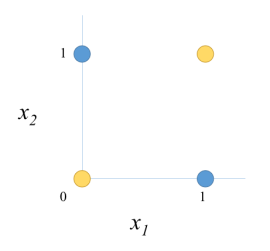
\includegraphics[width=.4\textwidth]{figures/chap2/xor-graph.png}
    \label{fig:xor}
\end{SCfigure}

Now let consider a 1-hidden-layer $\displaystyle FNN$ with activation function relu ($\displaystyle relu(x) = max(0, x)$), we can now specify $\displaystyle XOR$ function as:
\[ f(x; W_1, W_2, b_1, b_2) = W_2.max(0, W_1x + b_1) + b_2 \label{equation_xor} \]
We can now specify a solution to the $\displaystyle XOR$ problem. Let
\[ W_1 = 
\begin{bmatrix}
    1 & 1 \\
    1 & 1
\end{bmatrix}, \]

\[ b_1 =
\begin{bmatrix}
    0 \\
    -1
\end{bmatrix}, \]

\[ W_2 =
\begin{bmatrix}
    1 & -2
\end{bmatrix}, \]

and $\displaystyle b_2 = 0$. We can check the result by computing the value of \eqref{equation_xor} with the given input $\displaystyle X$ below:
\[ X = 
\begin{bmatrix}
    0 & 0 & 1 & 1 \\
    0 & 1 & 0 & 1
\end{bmatrix}, \]
where each column of $\displaystyle X$ is an input pair $\displaystyle (x_1, x_2)$,
\begin{align*}
    f(X; W_1, W_2, b_1, b_2) &= W_2.max(0, W_1x + b_1) + b_2 \\
    {} &= \begin{bmatrix}
            1 & -2
          \end{bmatrix}.max \left(0, 
            \begin{bmatrix}
                1 & 1 \\
                1 & 1
            \end{bmatrix} \begin{bmatrix}
                0 & 0 & 1 & 1 \\
                0 & 1 & 0 & 1
            \end{bmatrix} + \begin{bmatrix}
                0 \\
                -1
            \end{bmatrix}\right) + 0 \\
    {} &= \begin{bmatrix}
        1 & -2
      \end{bmatrix}.max \left(0, 
        \begin{bmatrix}
            0 & 1 & 1 & 2 \\
            0 & 1 & 1 & 2
        \end{bmatrix} + \begin{bmatrix}
            0 \\
            -1
        \end{bmatrix}\right) \\
    {} &= \begin{bmatrix}
        1 & -2
        \end{bmatrix}.max \left(0, 
        \begin{bmatrix}
            0 & 1 & 1 & 2 \\
            -1 & 0 & 0 & 1
        \end{bmatrix}\right) \\
    {} &= \begin{bmatrix}
        1 & -2
        \end{bmatrix}.\begin{bmatrix}
            0 & 1 & 1 & 2 \\
            0 & 0 & 0 & 1
        \end{bmatrix}\\
    {} &= \begin{bmatrix}
        0 & 1 & 1 & 0
        \end{bmatrix}
\end{align*}
We can see that the final result is exactly what we expected.


\subsection{Convolutional Neural Networks}
Convolutional Neural Networks (CNNs) are a specialized kind of feedforward neural networks for processing data that has a grid-like topology. This type of networks archives a considerable amount of success in many machine learning problem, from 1D data (time-series audio signal, etc) to 2D data (computer vision, etc). The most noticeable difference between CNNs and FNNs is that instead of using a matrix multiplication as FNN, CNNs use convolution operation. In the context of this thesis, we concentrate on the 2D convolution operation executed by two operators: a matrix which is the restricted portion of the receptive field and a matrix which is the set of learnable parameters (a.k.a. kernel). The kernel is spatially smaller than an image, but has the same number of channels. For example, if the image is composed of three (RGB) channels, the kernel height and width will be spatially small, but the depth extends up to all three channels. Usually, there is more than one kernel in the same convolutional layer, e.g. 16, 32, 64 kernels.

\textbf{Concrete Example.} Suppose that we have a input image $\displaystyle X$ with size \newline $\displaystyle 32 \times 32 \times 3$, a kernel $\displaystyle w$ with size $\displaystyle 5 \times 5 \times 3$, padding isn't used and stride is $1$. This kernel has $\displaystyle 5 * 5 * 3 = 75$ parameters to be learnt. We can convolve this filter by sliding it across all spatial positions of the input tensor and computing a dot product between a small chunk of $\displaystyle X$ and the filter $\displaystyle w$ at each position. The result will be an activation map, which in this case would have the dimensions $\displaystyle 28 \times 28$ (28 is the number of unique positions that a filter of 5 elements can be placed over an input of size 32) (An example of convolution operation is in figure \ref{fig:cnn}). In some cases, padding is used when users want to increase the spacial dimensions of the output (commonly the same as input tensor $\displaystyle X$). In addition, if there is no padding and stride 2 is used, output tensor has size of $\displaystyle 14 \times 14$. Finally, if kernel size is set to 64, input tensor $\displaystyle X$ executes convolution operation independently with these filters, and the final output has the shape of $\displaystyle 28 \times 28 \times 64$.

\begin{figure}[h!]
    \begin{center}
        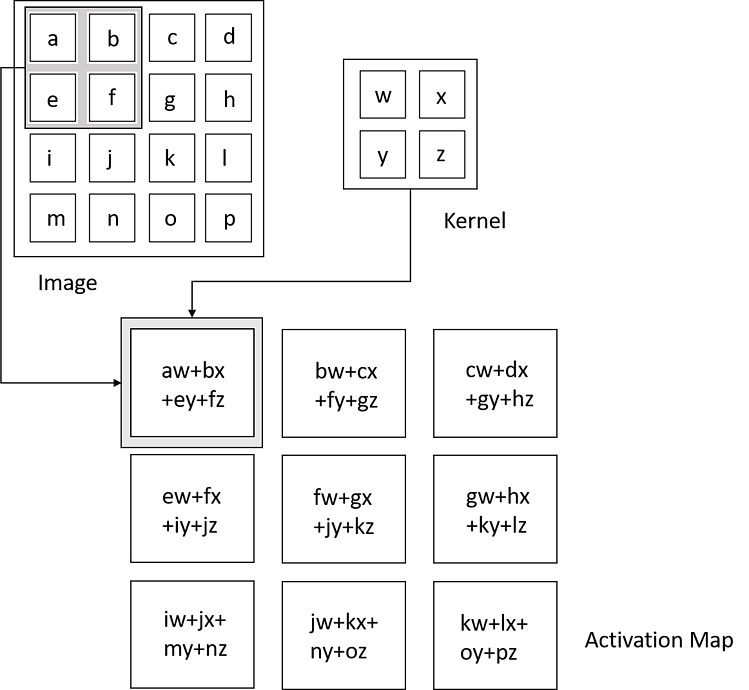
\includegraphics[width=0.7\textwidth]{figures/chap2/cnn.png}
        \caption{Convolution Operation \cite{dlbook}}
        \label{fig:cnn}
    \end{center}
\end{figure}

\textbf{General definition.} Formally, a convolutional layer for images (assuming input tensors with three spatial dimensions):
\begin{itemize}
    \item Has a $\displaystyle W_1 \times H_1 \times D_1$ tensor as input.
    \item Requires \textbf{4 hyperparameters}: The number of filter $\displaystyle K$, the spatial dimension $\displaystyle F$, the stride $\displaystyle S$, and the amount of padding on the borders of the input, $\displaystyle P$.
    \item The number of parameters of each filter is $\displaystyle F \times F \times D_1$ and one bias (if used bias), so with a set of $\displaystyle K$ filters, there is totally $\displaystyle K \times F \times F \times D_1$ weights and $\displaystyle K$ biases.
    \item The output is a tensor of size $\displaystyle W_2 \times H_2 \times K$, where $\displaystyle W_2 = (W_1 - F + 2P)/S + 1$, $\displaystyle H_2 = (H_1 - F + 2P)/S + 1$.
\end{itemize}

\section{Recurrent Neural Networks}
In this section, we introduce briefly Recurrent Neural Networks (RNNs), which is the type of neural networks mainly used in this work. RNNs show their significant performance in many problems where input data are in form of sequence, such as language model or time-series predictions. The original idea of RNNs comes from the sharing parameter mechanism, which is presented in CNNs. However, while CNNs is only capable of sharing parameter across a small number of neighbors, RNNs allow to share parameters through further neigbors, maybe hundred-length sequences.  

\subsection{Vanilla Recurrent Neural Networks}
Vanilla Recurrent Neural Network is the most basic and natural method when humans first think about applying recurrent mechanism in neural networks. In a Vanilla RNN, each output at index $\displaystyle t$ is a function of the output at index $\displaystyle t - 1$, except output at index $\displaystyle 0$ (it is usually zero-initialized or also learnable parameters). The typical function in RNN is:
\[ h_t = \tanh \left( W\begin{pmatrix} x_t \\ h_{t-1} \end{pmatrix} \right) \]

However, Vanilla RNNs have low performance on long sequence data, due to \textit{vanishing} and \textit{exploiding} gradient. Exploiding gradient, which means that gradient's value becomes too large through recurrent backpropagation (due to multiple multiplication with many greater-than-1 numbers), is rarely occured, but its consequence is also huge. Clipping gradient \cite{DBLP:Clipping-gradient} is an efficient solution for this problem. However, vanishing gradient can't be solved by this method. Vanishing gradient happens when a gradient is multipled by many \textit{absolutely-smaller-than-1} numbers and reaches zero, which leads to the reduction of the weight correspondant to this gradient.

\subsection{Long-Short Term Memory Neural Networks}
There are a number of variants of LSTM. In this work, we use the LSTM with "peephole connections" of Gers and Schmihuber (2000) \cite{Peephole-LSTM}, which makes use of information at the previous cell state to be a part of input of gate layers. The formula of LSTM is described by equations \eqref{equation-lstm-ft} to \eqref{equation-lstm-ht}

\[ f_t = \sigma(W_f[C_{t-1}, h_{t-1},x_t] + b_f) \label{equation-lstm-ft}\] 
\[ i_t = \sigma(W_i[C_{t-1}, h_{t-1},x_t] + b_i) \label{equation-lstm-it}\]
\[ \hat{C}_t = \tanh(W_c[C_{t-1}, h_{t-1},x_t]) \label{equation-lstm-Chat-t}\]
\[ C_t = f_t * C_{t-1} + i_t * \hat{C}_t \label{equation-lstm-Ct}\]
\[ o_t = \sigma(W_o[C_{t}, h_{t-1},x_t] + b_o) \label{equation-lstm-ot}\]
\[ h_t = o_t * \tanh(C_t) {equation-lstm-ht}\]


\section{Summary}
In summary, a typical workflow for applying a neural network in some context looks as follows:

\textbf{Data preparation.} First, obtain a dataset. For the purposes of this dissertation we have assumed that the dataset is made up of a set of pairs $\displaystyle (x, y)$ where $\displaystyle x$ is some input example and $\displaystyle y$ is a label. We then split the dataset into three folds, commonly a training, validation and test fold (common proportions could be 80\%, 10\%, 10\% respectively). We will use the training fold for optimizing the parameters with backpropagation, the validation fold for hyperparameter optimization, and the test fold for evaluation (discussed below in more detail).

\textbf{Data preprocessing.} Preprocessing the data can help improve convergence of neural networks. For images, common preprocessing techniques involve standardizing the data (subtracting the mean and dividing by the standard deviation individually for every input dimension of $\displaystyle x$), or at the very least subtracting the mean. It is critical to estimate these statistics only on the training data, and using these fixed statistics to process the validation and test data, as this appropriately simulates the deployment of the final system into a real-world application.

\textbf{Architecture design.} Next we must to decide on a family of architectures that we wish to explore. In our notation above, this amounts to designing the internals of the computation graph that makes up the function $\displaystyle f$. This stage is more of an art than a science, but we discuss a few common heuristics used in practice. It is common to process pixel data with convolutions and sequence data with recurrent networks. For the scale of the architecture, a very rough rule of thumb is that the full model should have approximately similar number of parameters as there are examples in the training dataset.

\textbf{Optimization.} A default recommendation is to use Adam \cite{article:Adam-optimization} for optimization, with learning rates of approximately $\displaystyle 1e3$, the coecient of first moment of $\displaystyle 0.9$ and second moment $\displaystyle 0.99$. It is often beneficial to anneal the learning rate during the course of training by approximately a factor of $\displaystyle 100$ by the very end of training, but it si common to decay the first time only after half of the training is finished. As a a good sanity check to help debug the code, it is a good idea to try to
overfit a single batch of data (reaching zero training loss) before optimizing over the full training set.

\textbf{Hyperparameter optimization.} The optimization with stochastic gradient can be seen as an inner loop of the optimization, while hyperparameter optimization is the outer loop that determines good values of hyperparameters that are dicult or impossible to backpropagate into (such as the learning rate, or the number of units in the hidden layers). This process consists of sampling hyperparameters from some search range (it is best to sample at random rather than along the grid), optimizing the model, and evaluating the model on the validation fold. The final best model is the one that achieves the best validation performance.

\textbf{Evaluation.} Once we identify the best trained model (with the lowest validation loss), we evaluate the model a single time on the test set and report the performance. Consistent improvements can always be obtained by using model ensembles, which average the results of evaluating multiple models trained from different initializations or with dfferent hyperparameters.
